\documentclass[9pt,twocolumn,twoside]{../../styles/osajnl}
\usepackage{fancyvrb}
\journal{i524} 

\title{Heroku}

\author[1,*, +]{Yatin Sharma}

\affil[1]{School of Informatics and Computing, Bloomington, IN 47408, U.S.A.}

\affil[*]{Corresponding authors: yatins@indiana.edu}

\affil[+]{HID - S17-IR-2034}

\dates{Paper-002, \today}

\ociscodes{Heroku, PaaS, Dyno, Dyno Manifold, Logplex, Toolbelt client, Procfile.}

% replace this with your url in github/gitlab
\doi{\url{https://github.com/cloudmesh/sp17-i524/tree/master/paper2/S17-IR-2034/report.pdf}}


\begin{abstract}
	Heroku is a web application hosting platform-as-a-service cloud  that enables
	developers to build and deploy application. It supports multiple programming
	languages including Ruby, Java, Node .js and Python. It is a simple and modular
	platform that allows developers to focus less on infrastructure/deployment and
	focus more on coding. 
	\newline
\end{abstract}

\setboolean{displaycopyright}{true}

\begin{document}

\maketitle

\section{Introduction}
	Heroku\cite{Heroku} is Platform as a Service(Paas)\cite{PaaS} that enables us
	to build and deploy applications in various programming language including Java,
	Python, Ruby, etc. It allows us to deploy web applications seamlessly as well as
	monitor and share with other developers instantly. It is enables rapid
	application development for the cloud, using the underlying platform
	infrastructure and software add-ons to build, deploy and monitor large and
	scalable web applications. It is built on top of Amazon Web Services and is owned
	by Salesforce.com \cite{Salesforce}. 
	

	
\section{Benefits}
	Heroku is language agnostics and provides great flexibility in choosing an
	appropriate programming language to develop the web application. It has core
	support for Clojure, Ruby, Java, Python, Node.js, Scala and Play, Go, and PHP.
	Apart from these, any other language can also be supported by using a feature
	called buildpacks. Heroku provides a lot of flexibility in managing the
	applications after deployment using the Heroku command line tool running on the
	client machine or on the Heroku Infrastructure. Heroku uses Git\cite{Git} as the
	means for deploying applications to its servers. Being owned by
	Salesforce.com\cite{Salesforce}, it has a feature called Heroku Connect enabling
	interaction between the applications and Salesforce API.

	\section{Architecture}
	The Heroku architecture consists of platform stack containing various runtime
	libraries, OS, and underlying infrastructure. A Heroku application can be
	thought of a multiple processes, each consuming resources like a normal UNIX
	process, that run on the Heroku Dyno manifold. Heroku defines each process
	through configuration file called Procfile- which is a text file, placed in root
	of the application and contains the format describing how the application will
	run. Fig. 1. below describes the high level architecture of the Heroku platform.
	
	\begin{figure}[htbp]
		\centering
		\fbox{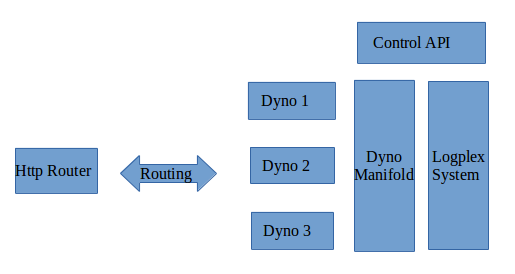
\includegraphics[width=\linewidth]{images/Heroku.png}}
		\caption{High Level Architecture of Heroku platform}
		\label{fig:Herokul-arch}
	\end{figure}

	


\subsection{Process Management}
	
	The unit of work in Heroku framework is called Dyno. It can be thought of as
	packaged running version of the code that the application interacts with. Dynos
	are responsible for receiving web requests, writing an output and connecting to
	application resources such as databases. They are fully isolated containers
	running on the Dyno Manifold, which is the building block for execution
	environment. Dyno Manifold is responsible for process management,
	isolation,scaling, routing, distribution that are necessary for to run the web
	and worker processes. It is also fault tolerant and distributed in nature. If
	any dynos fails, the manifold restarts them automatically, hence removing a lot
	of maintenance hassles.Dynos are capable of serving many request per second and
	execute in complete isolation from each other. Each dyno gets its own virtual
	environment that it can use to handle its own client requests. Dynos use LXC 
	to provide container like behavior to achieve complete isolation from one 
	another.There is a memory restriction of 1.5 GB per dyno, beyond which the 
	dyno is rebooted with a Heroku error which could lead to a memory leak.

\subsection{Execution Flow}
	Process type is the declaration of the command that defines the structure to be
	used while instantiating a process. Heroku has two process types- web process,
	which is responsible for handling HTTP client requests and the worker process,
	which is responsible for executing other tasks such as customer jobs of running
	background jobs and queuing tasks.



\subsection{Logging Architecture}
	Heroku logplex system provides a flexibility facility by giving us an overall
	view of the application runtime behavior. It forms the basis of the Heroku
	logging  infrastructure. It routes log streams form various sources into single
	output( for example archival system). The logplex system keeps the most recent
	data ( typically 1500 logs) that are important to extract relevant information
	from the application  being run.

\subsection{Http Routing}
	Routing Mesh are responsible for routing the web requests to the appropriate
	web process dyno. It is also responsible for seeking the application’s web dynos
	within the dyno manifold and forwarding the HTTP web requests to one of them.
	The routing mesh uses a round robin algorithm to distribute the request acroos
	various dynos. Since the dynos could be running in distributed manner, the
	routing mesh manages the access and routing internally and none of the dynos are
	statically addressable. Heroku also supports multithreaded and asynchronous
	application, accepting many network connections to process client requests.

\subsection{Heroku Interfaces}
	
	Heroku provides the developer with the flexibility to control various aspects 
	of the application through various control surfaces such as process management,
	routing, logging, scaling, configuration, and deployment. These are available 
	as a command-line interface (CLI), a web-based console, and full REST API.

\section{Addons}

	Heroku supports vast amount of third party addons\cite{Addons} that any Heroku
	user can instantly provision as an attachable resource for their application.
	For example, if the application needs a PostgreSQL\cite{PostgresSQL} database, 
	it can be done in Heroku. Addons work through Heroku’s environment variables. 
	Each time an addon is added to the application, the application will
	automatically be assigned new environment variables which specify any
	configurations required to interact with the new addon. Just like Dynos, Addons
	are easy to add, up-grade, downgrade, and remove without requiring any downtime
	for the applications.

\section{Heroku Platform API}
	Heroku platform API is a tool that allows to call Heroku platform services,
	create applications, and plug in new add-ons by simply using HTTP. It gives the
	developers complete control over their application. The three components that
	define the behavior of the API are : 1)Security 2)Schema 3)Data. The client
	accesses the API using standard methods defined for HTTP. The API then acts on
	the request and returns the result in JSON format.

\section{Security}
	Heroku employs various measures to ensure that the application and data stores
	within the platform are secure from external attacks,thefts and hacks. Heroku
	enforces SSH\cite{SSH} protocol to encrypt the source code while they are
	getting pushed into the Heroku environment. Any application that runs on Heroku
	is in complete isolation from another, so that no two application can see
	each other getting executed. It also restricts applications from making local
	network connection between hosts. It enables data security by keeping the data
	in access controlled databases.


\section{Getting started}
	
	There are few prerequisites that we need to perform before we can start using
	Heroku: 1) Get Heroku account 2) Install Heroku toolbelt client\cite{Toolbelt} 
	3) Set up SSH for the user account. Heroku toolbelt is the client software
	required to work with the Heroku platform and contains the following component:
	Heroku Client, Foreman and Git. Step-by-step procedures to download, install 
	and get started with Heroku can be found on-line.\cite{Tutorial}

\section{Conclusion}

	Heroku offers a Platform as a Service (PaaS) in which the servers and
	filesystems are completely abstracted away. It gives provides an environment
	where pushing the code and basic configuration can get an application running.
	It provides a complete developer experience and an application runtime. It
	manages all that in scalable and highly maintainable fashion. It's logging
	service as well as instant scaling power allows scaling up to support demand
	from users, and scaling down when high straffic has stopped.

\section*{Acknowledgements}

	The author thanks Prof. Gregor von Laszewski for his technical guidance.

% Bibliography

\bibliography{references}

\end{document}
